% !TEX program = xelatex
\documentclass{beamer}
\usetheme{compostela}

%%%%%%%%%%%%%%%%%%%%%%%%%%%%%%%%%%%%%%%%%%%%%%%%%%%%%%%%%%%%%%%%%%%%%%%%%%%%%%%%
%%%%%%%%%%%%%%%%%%%%%%%%%%%% Talk Configuration %%%%%%%%%%%%%%%%%%%%%%%%%%%%%%%%

\newcommand{\TalkPlace}{CMS Masterclass}
\newcommand{\TalkAuthor}{Marcos Romero Lamas}
\newcommand{\TalkAuthorShort}{Marcos Romero Lamas}
\newcommand{\TalkTitle}{Aceleradores e \\detectores de \\partículas}
\newcommand{\TalkTitleShort}{Aceleradores e detectores de partículas}
\newcommand{\TalkInstitute}{IGFAE}
\newcommand{\TalkDate}{11 de marzo}
\newcommand{\TalkDateNumber}{2021/03/11}

%%%%%%%%%%%%%%%%%%%%%%%%%%%%%%%%%%%%%%%%%%%%%%%%%%%%%%%%%%%%%%%%%%%%%%%%%%%%%%%%


\newenvironment{variableblock}[3]{%
  \setbeamercolor{block body}{#2}
  \setbeamercolor{block title}{#3}
  \begin{block}{#1}}{\end{block}}

\usepackage{xmpmulti} % animate...
\usepackage{animate}


\usepackage{pdfcomment}
\newcommand{\pdfnote}[1]{\marginnote{\pdfcomment[icon=note]{#1}}}



\begin{document}



%%%%%%%%%%%%%%%%%%%%%%%%%%%%%%%%%%%%%%%%%%%%%%%%%%%%%%%%%%%%%%%%%%%%%%%%%%%%%%%%
%%%%%%%%%%%%%%%%%%%%%%%%%%%%% TITLE PAGE & CONTENTS %%%%%%%%%%%%%%%%%%%%%%%%%%%%
%%%%%%%%%%%%%%%%%%%%%%%%%%%%%%%%%%%%%%%%%%%%%%%%%%%%%%%%%%%%%%%%%%%%%%%%%%%%%%%%

\begin{frame}[plain,backgroundpicture=gpx/cms_higgs_43,overlaytitlepage=0.9]
  \begin{minipage}[b][\textheight][b]{5cm}
    
\includegraphics[height=0.35cm]{logos/maeztu_bw}\hspace{1mm}
    
\includegraphics[height=0.35cm]{logos/igfae_bw}\hspace{1mm}
    
\includegraphics[height=0.35cm]{logos/usc_bw}\hspace{1mm}
    
\includegraphics[height=0.35cm]{logos/xunta_bw}\hspace{1mm}
  \end{minipage}
\end{frame}

\begin{frame}[plain,backgroundpicture=gpx/cms_higgs_43,overlaytoc=0.9]
  \addtocounter{framenumber}{-1}
  \hspace*{7.3cm}\begin{minipage}{8cm}
    \tableofcontents
  \end{minipage}
\end{frame}

%%%%%%%%%%%%%%%%%%%%%%%%%%%%%%%%%%%%%%%%%%%%%%%%%%%%%%%%%%%%%%%%%%%%%%%%%%%%%%%%



\section{O CERN}



\subsection{Orixe}



\begin{frame}
  \frametitle{noframetitle}
  \begin{tikzpicture}[overlay, remember picture]
  \node at (9.8,-4.0)
  {\animategraphics[width=0.4\textwidth,autoplay,loop]{1}{gpx/cern-states/out-}{0}{9}};
  \node at (9.5,0.5) {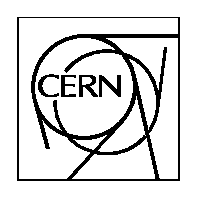
\includegraphics[width=2cm]{gpx/cern_logo.eps}};
  \end{tikzpicture}

  \begin{columns}
  \begin{column}{0.6\textwidth}
  \begin{itemize}
    \item Despois da Segunda Guerra Mundial, varios estados europeos uníronse para
    crearen un gran laboratorio común de investigación nuclear con propósito
    pacífico
    \item No ano 1964 nace o CERN: \emph{Conseil Européen pour la Recherche Nucléaire}
    \item Esta sito na cidade de Xenebra, en Suíza
    \item É o maior laboratorio de física do mundo
    \end{itemize}
  \end{column}
  \begin{column}{0.35\textwidth}
  \end{column}
  \end{columns}

\end{frame}



\begin{frame}[default, b, backgroundpicture=gpx/all_cern_states.pdf]
  \frametitle{noframetitle}
  A día de hoxe o CERN conta con:

  25 países membros {\color{scqblue} $\bullet$} 
  600 universidades {\color{scqblue} $\bullet$} 
  12000 científicos {\color{scqblue} $\bullet$} 
  70 nacionalidades
\end{frame}



\subsection{Obxectivo}



\begin{frame}[default, t]
  \frametitle{noframetitle}

  O obxectivo do CERN é o desenvolvemento da ciencia básica, explorando as
  preguntas máis fundamentais da natureza:\\[1cm]

  \centering
  \hspace*{-1cm} {\color{scqblue} \Huge \fontspec{SignPainter} Que é a materia?}

  \hspace*{3cm} {\color{scqgreen} \LARGE \fontspec{SignPainter} Cal é a súa orixe?}

  \hspace*{0cm} {\color{scqred} \LARGE \fontspec{SignPainter} Por que hai tres xeracións de \emph{quarks}?}

  {\color{scqindigo} \large \fontspec{SignPainter} Como está unida?}

  \hspace*{6cm} {\color{scqgreen} \Large \fontspec{SignPainter} Gravidade cuántica?}

  \hspace*{-5cm} {\color{scqblue} \LARGE \fontspec{SignPainter} Por que hai catro interaccións?}

  \hspace*{4cm} {\color{scqpink} \Huge \fontspec{SignPainter} Que é a materia escura?}

  \hspace*{-2cm} {\color{scqorange} \LARGE \fontspec{SignPainter} Por que as partículas teñen masas tan distintas?}

  \hspace*{-0cm} {\color{scqpurple} \LARGE \fontspec{SignPainter} Diferencias entre bosóns e fermións: supersimetría?}

\end{frame}



\begin{frame}
  \frametitle{Que precisamos?}

  \begin{columns}
  \begin{column}{0.45\textwidth}

    \begin{block}{Aceleradores}
    Máquinas poderosas quen de acelerar partículas ata enerxías extremadamente
    altas para levalas a colisionar con outras partículas 
    \end{block}

    \begin{block}{Detectores}
    Instrumentos xigantescos que rexistran as partículas producidas nas
    colisións, seguen as súas trazas e as identifican
    \end{block}
  \end{column}

  \begin{column}{0.45\textwidth}
    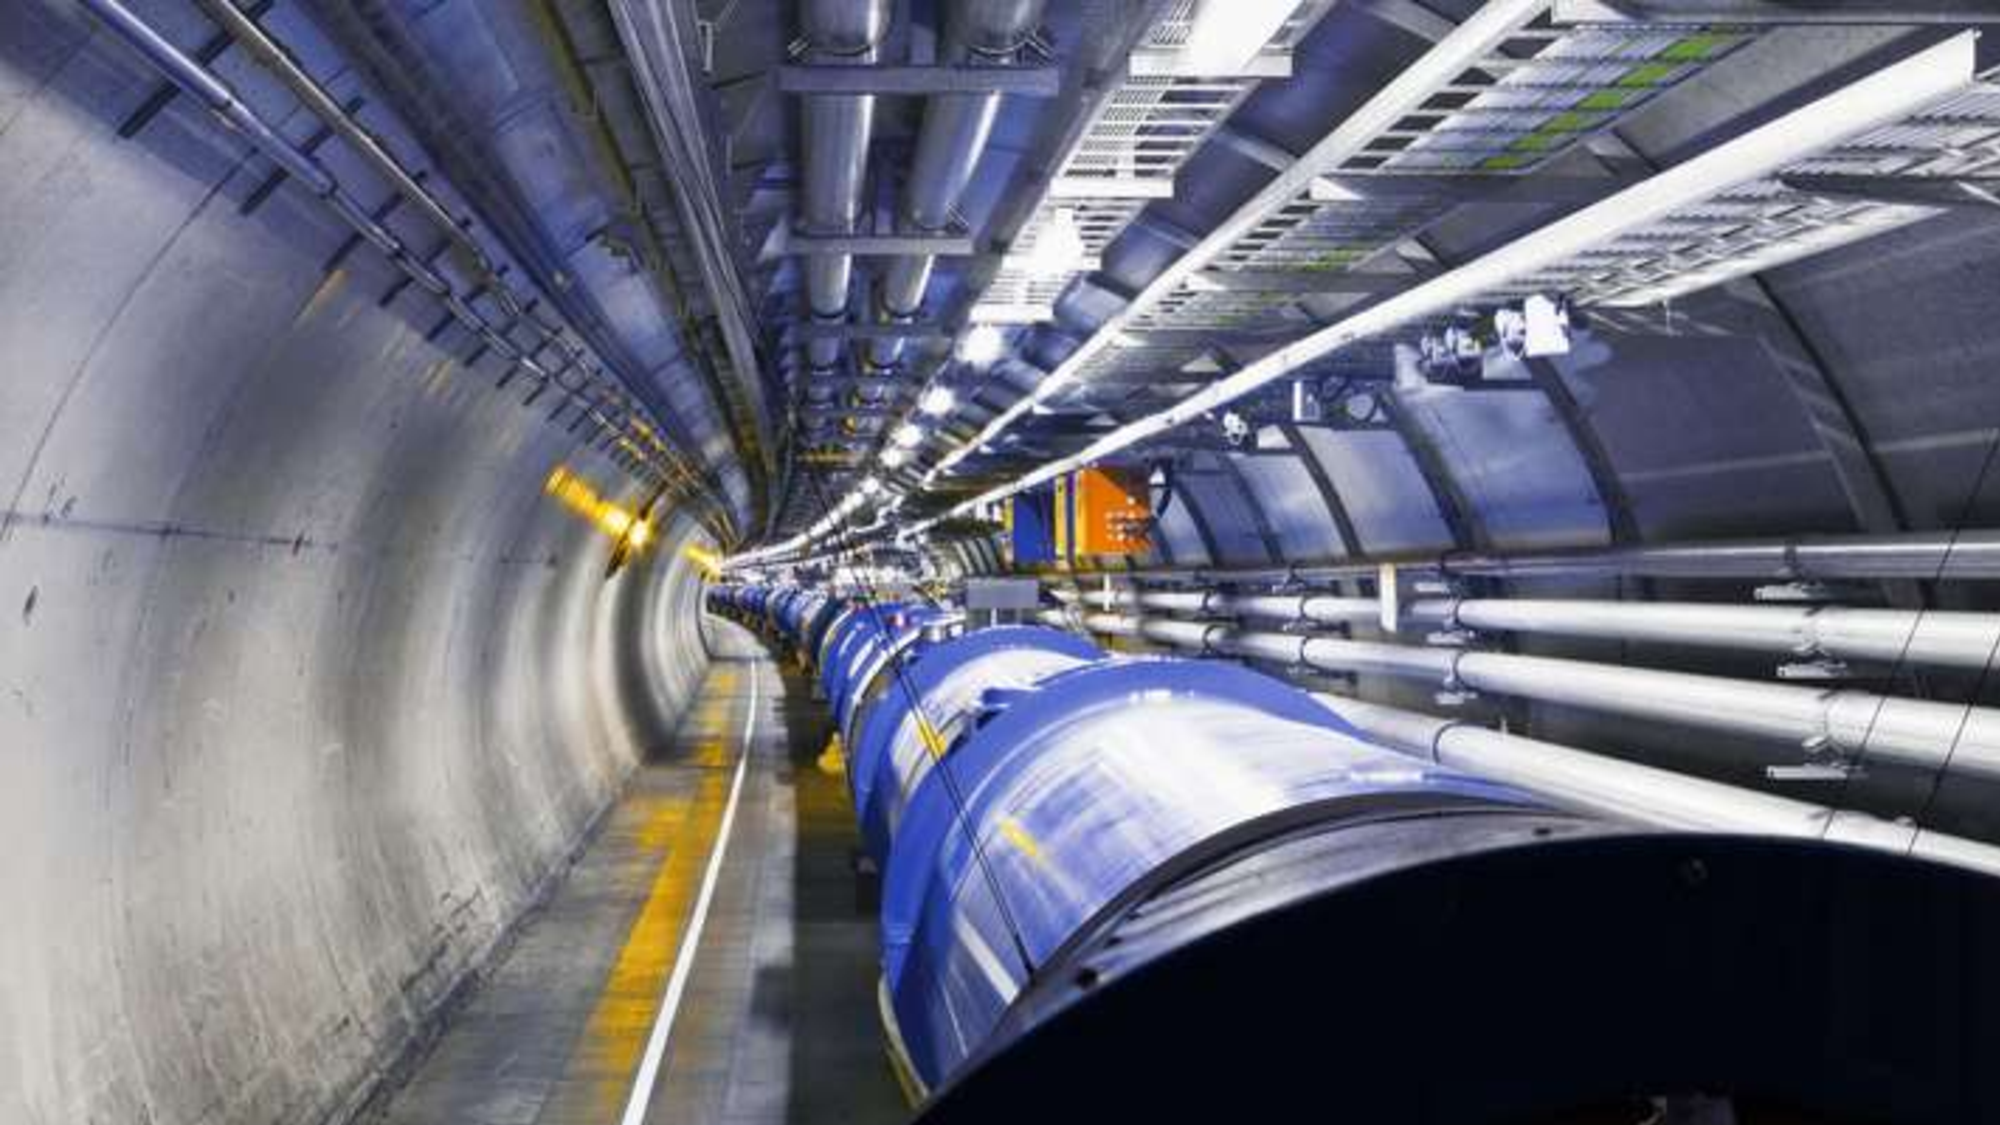
\includegraphics[width=\columnwidth, page=1]{gpx/examples.pdf}\\[5mm]
    \includegraphics[width=\columnwidth, page=3]{gpx/examples.pdf}
  \end{column}
  \end{columns}

\end{frame}




\begin{frame}
  \frametitle{Que precisamos?}

  \begin{columns}
  \begin{column}{0.45\textwidth}

    \begin{block}{Ordenadores}
    Permítennos recoller, almacenar, distribuir e analizar a gran cantidade de
    datos producidas polos detectores
    \end{block}

    \begin{block}{Persoas}
    Precísanse de enormes colaboracións internacionais de científicos, 
    enxeñeiros, técnicos e persoal de apoio para poder deseñar, construir e 
    sacar proveito destas máquinas tran complexas
    \end{block}
  \end{column}

  \begin{column}{0.45\textwidth}
    \includegraphics[width=\columnwidth, page=4]{gpx/examples.pdf}\\[5mm]
    \includegraphics[width=\columnwidth, page=2]{gpx/examples.pdf}
  \end{column}
  \end{columns}

\end{frame}



\subsection{LHC}



\begin{frame}[default, dark, t, backgroundpicture=gpx/lhc-earth.pdf]
  \frametitle{noframetitle}
  \begin{itemize}
    \item O LHC, \emph{Large Hadron Collider}, é o experimento máis grande co
    que o CERN conta até o momento
    \item Ten 27 km de circunferencia --- 8.6 km de raio
    \item Atópase soterrado unha media de 100 m baixo terra
    \item Conta con 4 detectores principais:
  \end{itemize} 

\end{frame}



%\begin{frame}[default]
%  \frametitle{Os catro detectores}
%
%  \centering
%
%  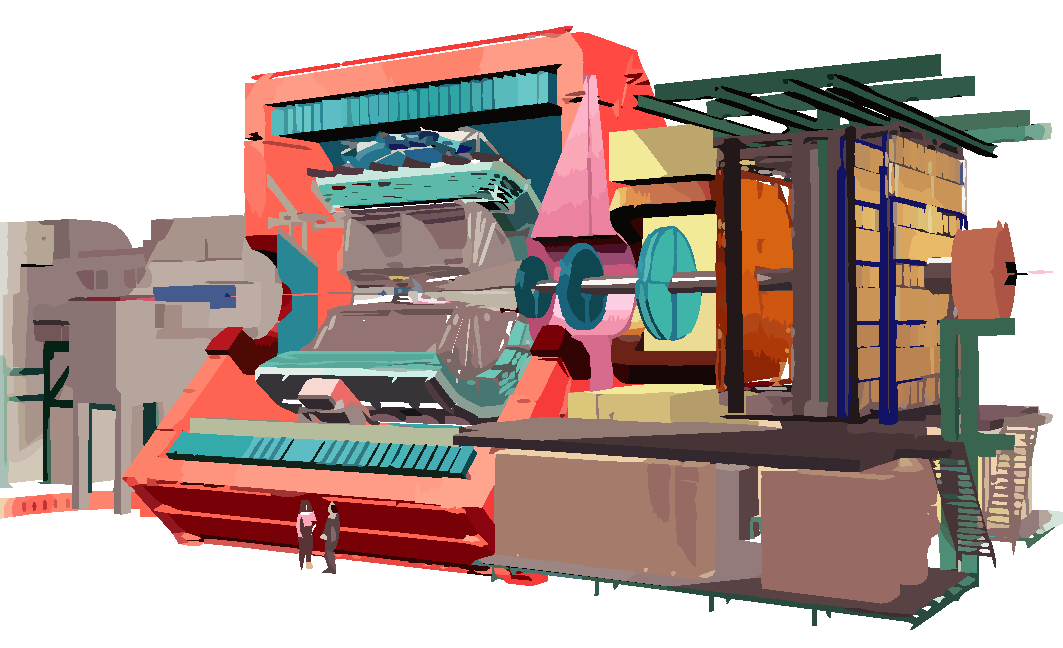
\includegraphics[width=0.3\textwidth,page=1]{gpx/3d_detectors}
%  \hspace*{1cm}
%  \includegraphics[width=0.3\textwidth,page=2]{gpx/3d_detectors}\\
%  ALICE \hspace*{3cm} ATLAS
%
%  \vspace*{5mm}
%
%  \includegraphics[width=0.3\textwidth,page=3]{gpx/3d_detectors}
%  \hspace*{1cm}
%  \includegraphics[width=0.3\textwidth,page=4]{gpx/3d_detectors}\\
%  CMS \hspace*{4cm} LHC$b$
%
%
%\end{frame}




\begin{frame}[default]
  \frametitle{noframetitle}
  
  \centering
  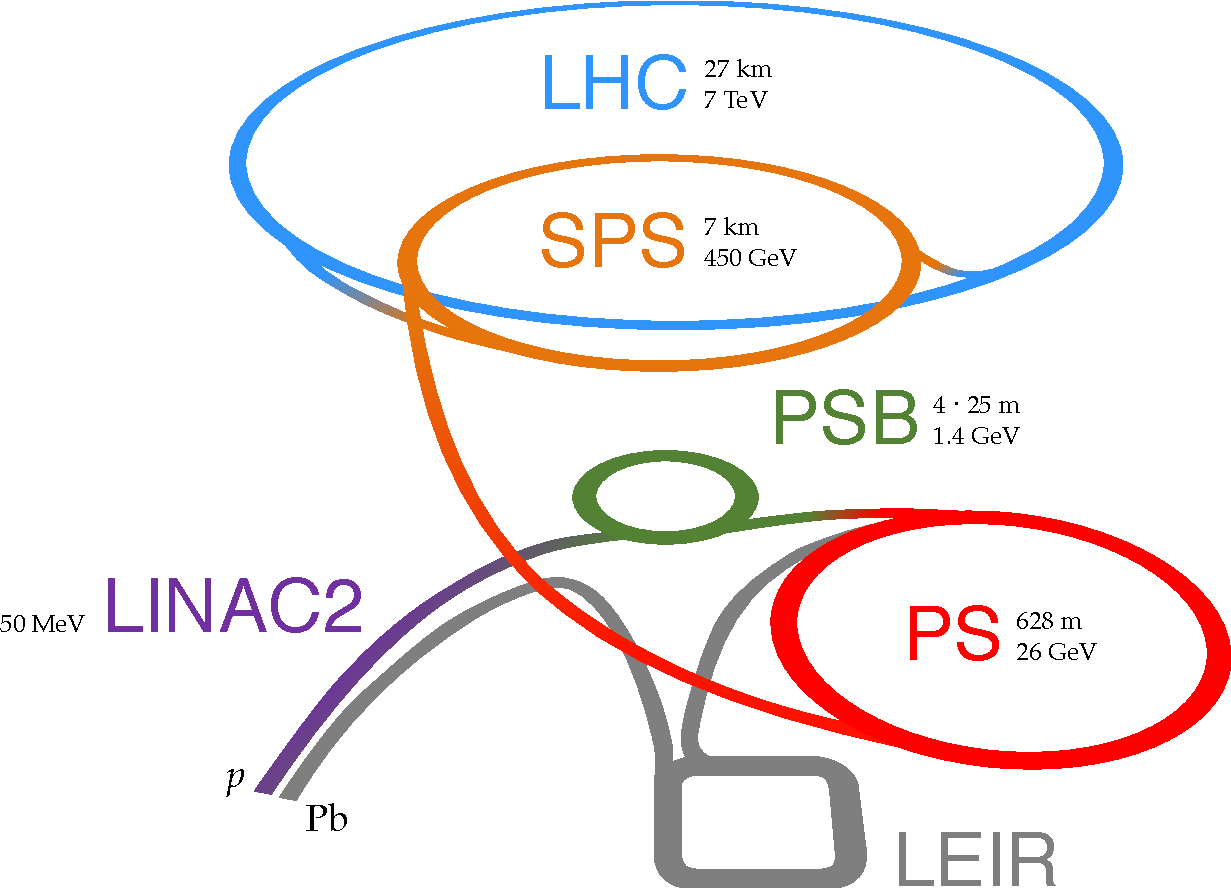
\includegraphics[width=0.8\textwidth]{gpx/lhc-chain.pdf}

\end{frame}



\begin{frame}[default]
  \frametitle{noframetitle}

  Estes experimentos teñen dimensións enormes:

  \bigskip

  \begin{columns}
  \begin{column}{0.45\textwidth}
    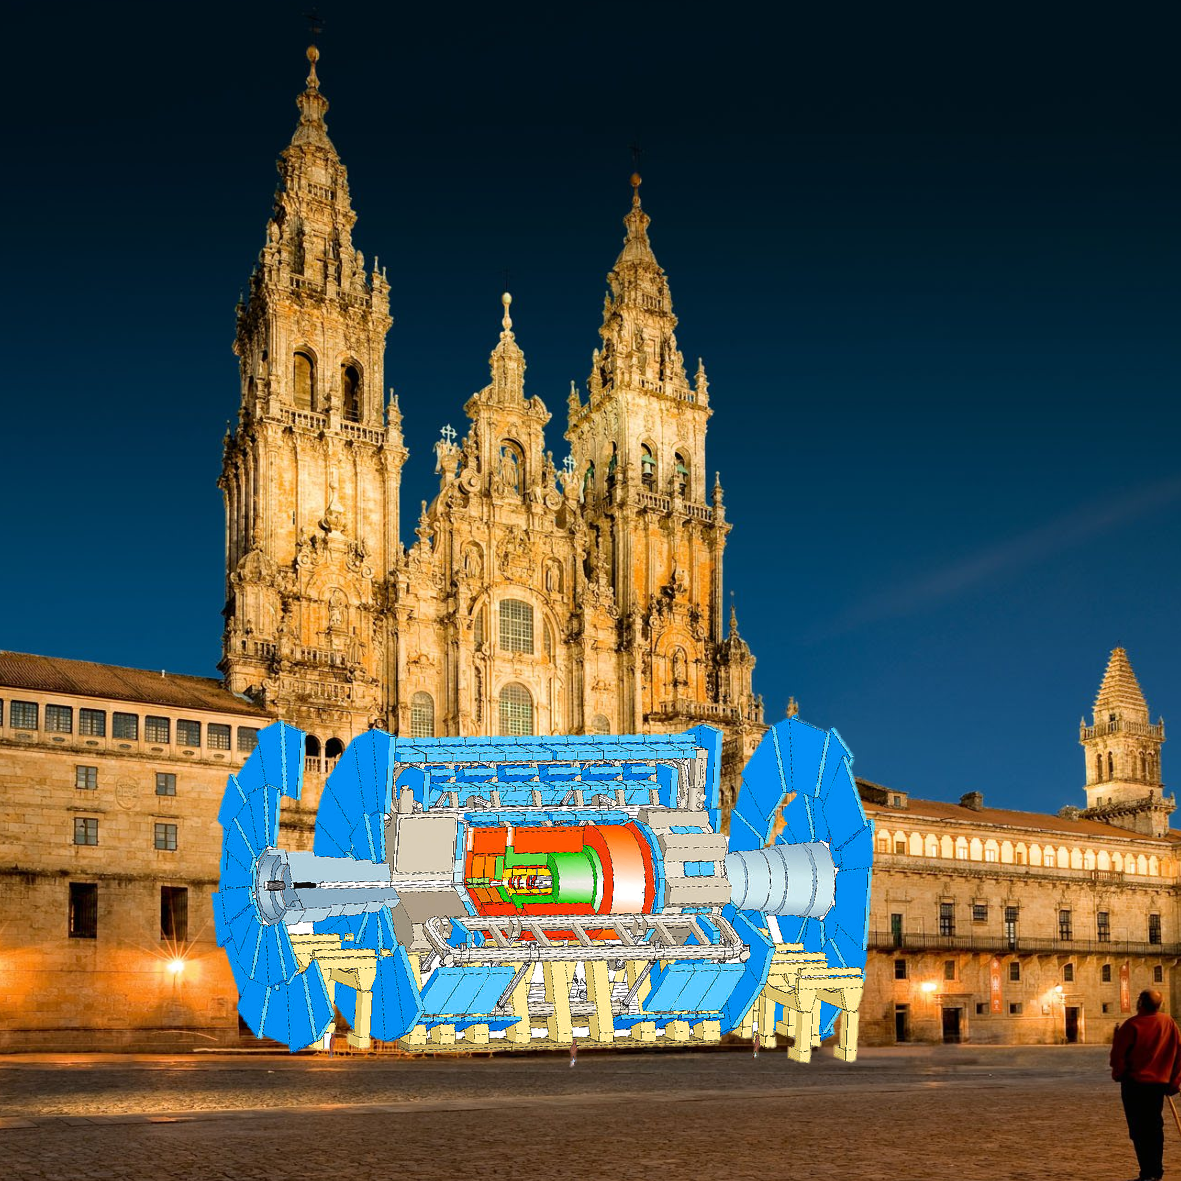
\includegraphics[width=\textwidth, page=1]{gpx/size_examples.pdf}
  \end{column}
  \begin{column}{0.45\textwidth}
    \includegraphics[width=\textwidth, page=2]{gpx/size_examples.pdf}
  \end{column}
  \end{columns}

\end{frame}


\begin{frame}[default, backgroundpicture=gpx/dvd_stack.pdf]
  \frametitle{Algúns números}
  \begin{columns}
  \begin{column}{0.65\textwidth}
    \begin{itemize}
      \item O \textbf{maior} dos detectores é \textbf{ATLAS}, con \textbf{25
      m} de alto
      \item A temperatura do interior do tubo é de $\mathbf{3}$ \textbf{K}, máis
      frío que o baleiro do universo
      \item Rexístranse $\mathbf{\sim 10^6}$ de colisións cada segundo.
      \item En \textbf{10 horas} de funcionamento, os protóns percorren o
      equivalente a ir ata \textbf{Neptuno e voltar}
      \item Cada feixe de protóns colisiona a \textbf{7 TeV}, o equivalente a 
      $\mathbf{5\times 10^9} $\textbf{pilas} de $1.5$ V / feixe
      \item Cada ano producen $\mathbf{15\times 10^6}$ de GiB de datos: 
      $\sim 20$ millons de DVDs
      \item LHC debe procesar \textbf{40 TiB de datos/segundo}; Facebook
      tan 'só' $\sim 4000$ TiB/día
      \item A análise dos datos precisa unha potencia de cálculo
      equivalente a $\mathbf{10^5}$ \textbf{CPUs} das máis rápidas
    \end{itemize} 
  \end{column}
  \begin{column}{0.3\textwidth}
  \end{column}
  \end{columns}

\end{frame}



\section{CMS}



\subsection{O segundo maior detector}



\begin{frame}
\frametitle{noframetitle}

\begin{columns}[T]
  \begin{column}{0.35\textwidth}
  \begin{center}
    
\includegraphics[scale=0.2]{gpx/cms_logo.pdf}
  \end{center}
  \begin{itemize}
    \item \emph{Compact Muon Solenoid}
    \item +5000 persoas
    \item 206 institutos
    \item 47 países
    \end{itemize}
  \end{column}


  \begin{column}{0.55\textwidth}
    \begin{itemize}
    \item Ten unhas dimensións de \\ 21 m $\times$ 15 m $\times$ 15 m
    \item $4$ T de campo magnético interior; $10^{15}$ veces o da Terra
    \item 12500 t de ferro; o dobre da Torre Eiffel
    \item Imán superconductor polo que circulan 18000 A de corrente; suficiente
    para cargar 8000 móviles en 30 minutos.
    \end{itemize}
    
    \bigskip 

    \begin{itemize}
    \item Descubriu o 4 de xullo de 2012 o bosón de Higgs, xunto con ATLAS
    \item Trátase dun detector de propósito xeral
    \end{itemize}
  \end{column}

\end{columns}

\end{frame}



\begin{frame}
\frametitle{noframetitle}
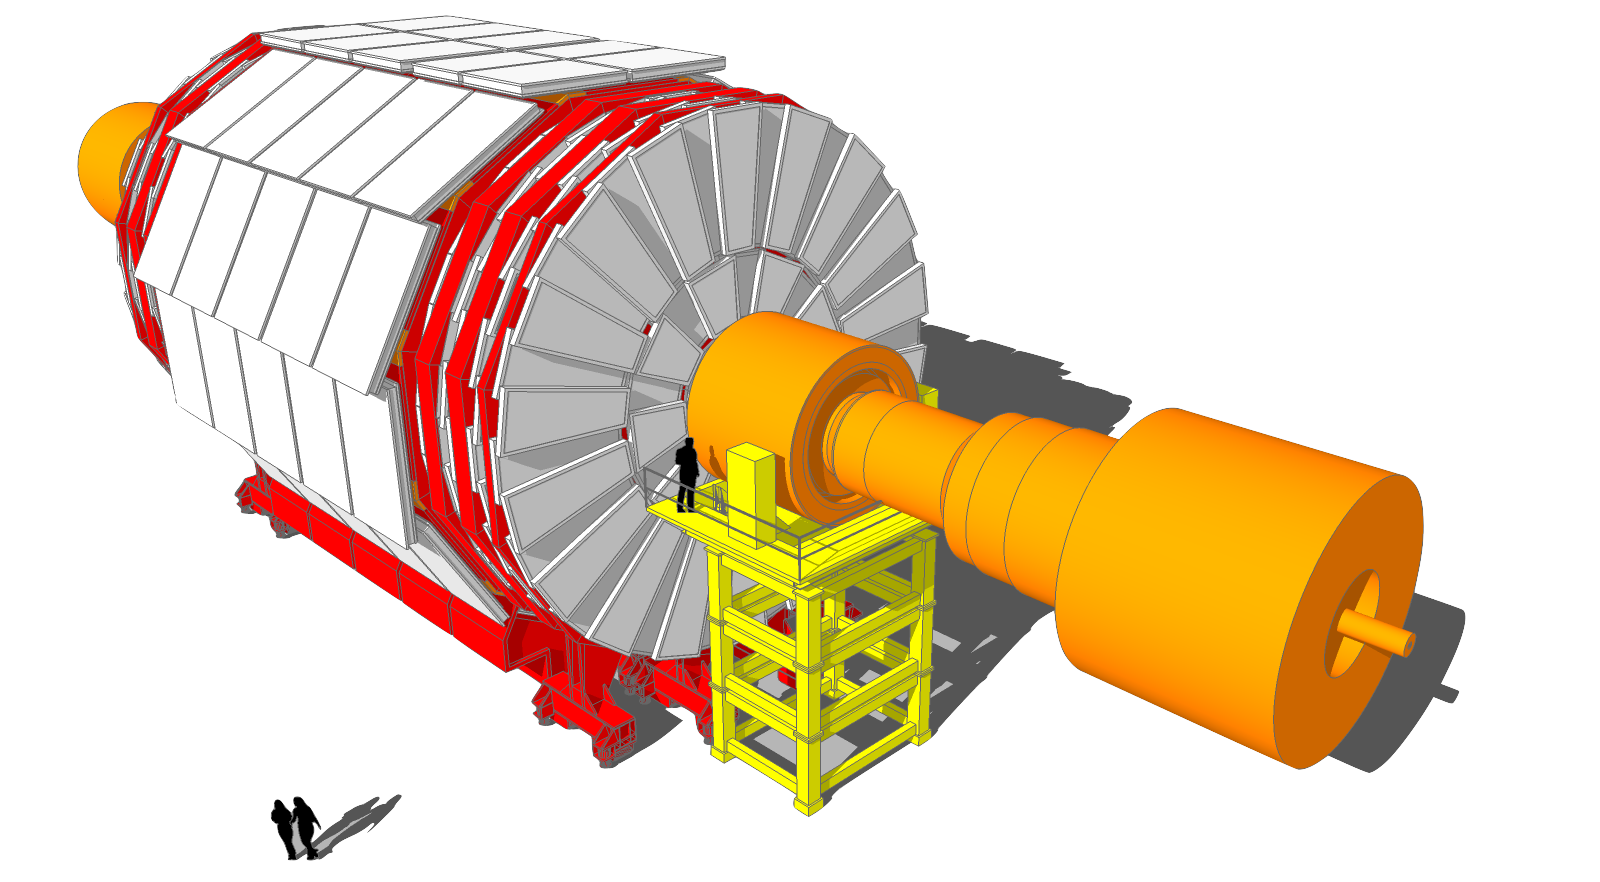
\includegraphics[width=\textwidth]{gpx/cms_3d_close.png}
\end{frame}



\addtocounter{framenumber}{-1}



\begin{frame}
\frametitle{noframetitle}
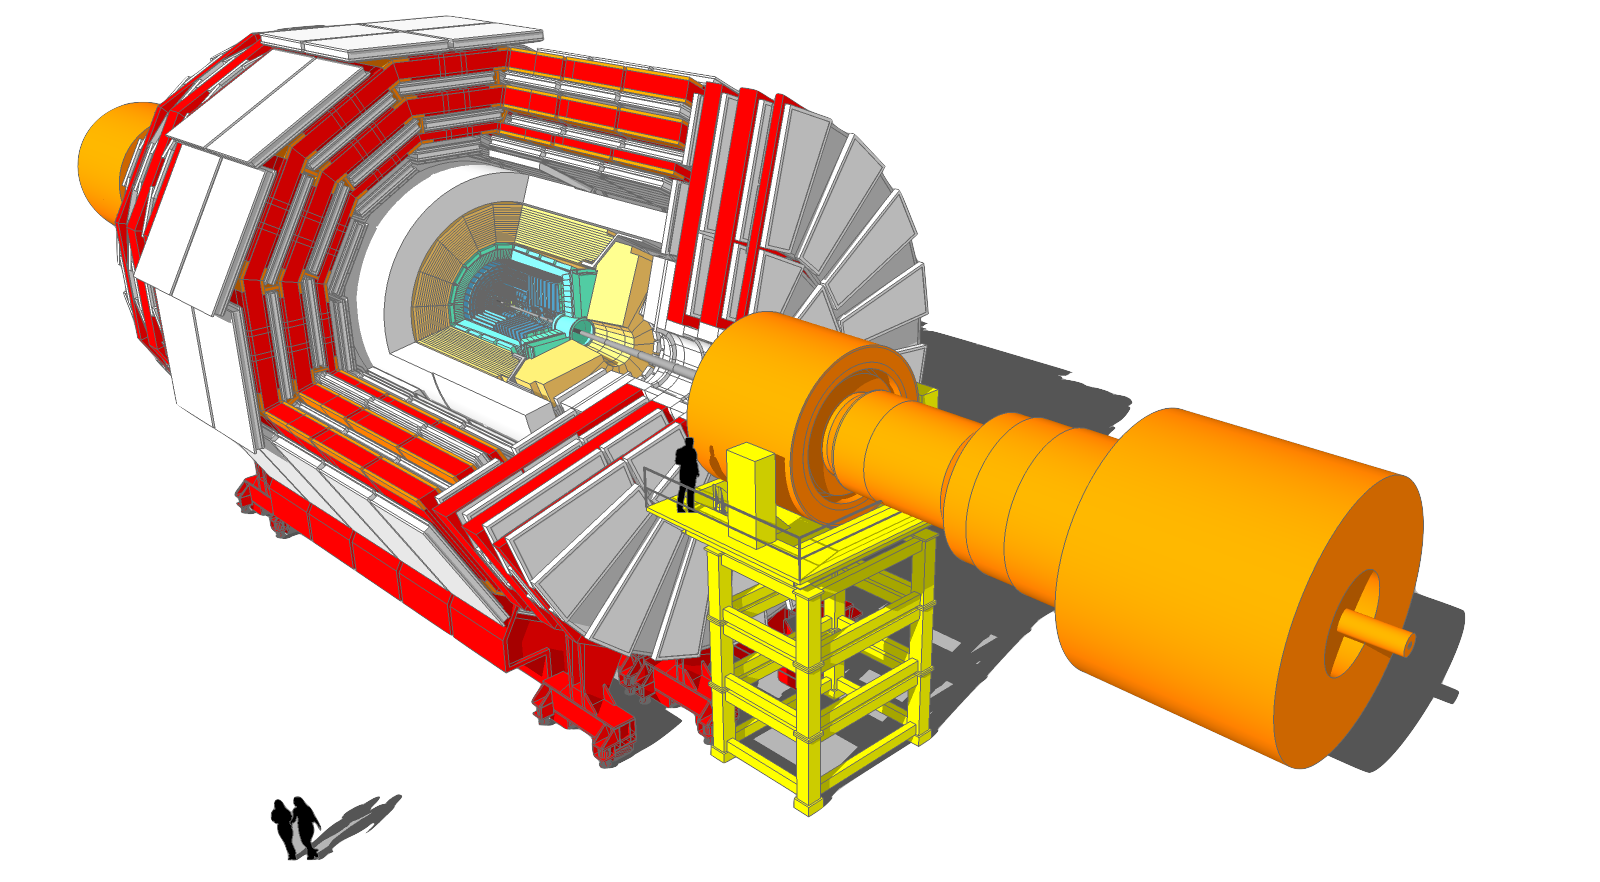
\includegraphics[width=\textwidth]{gpx/cms_3d_open.png}
\end{frame}



\subsection{Detectando ás partículas}



\begin{frame}
\frametitle{noframetitle}
\footnotesize

\begin{tikzpicture}[overlay, remember picture]
\node at (5.99,-3.0) {{\only<1,8>{\includegraphics[height=1.2\textheight]{gpx/CMS.pdf}}}};
\node at (5.99,-3.0) {{\only<2>{\includegraphics[height=1.2\textheight]{gpx/CMS-muon.pdf}}}};
\node at (5.99,-3.0) {{\only<3>{\includegraphics[height=1.2\textheight]{gpx/CMS-electron.pdf}}}};
\node at (5.99,-3.0) {{\only<4>{\includegraphics[height=1.2\textheight]{gpx/CMS-foton.pdf}}}};
\node at (5.99,-3.0) {{\only<5>{\includegraphics[height=1.2\textheight]{gpx/CMS-proton.pdf}}}};
\node at (5.99,-3.0) {{\only<6>{\includegraphics[height=1.2\textheight]{gpx/CMS-neutron.pdf}}}};
\node at (5.99,-3.0) {{\only<7>{\includegraphics[height=1.2\textheight]{gpx/CMS-neutrino.pdf}}}};
\end{tikzpicture}

\begin{tikzpicture}[overlay, remember picture]
\node at (1.00,-4.00) {{\only<1>{\emph{tracker} interno}}};
\node at (2.25,+0.00) {{\only<1>{calorímetro}}};
\node at (2.25,-0.25) {{\only<1>{electrónico}}};
\node at (2.25,-0.50) {{\only<1>{ECAL}}};
\node at (3.50,-5.25) {{\only<1>{calorímetro hadrónico}}};
\node at (3.50,-5.50) {{\only<1>{HCAL}}};
\node at (5.00,+0.75) {{\only<1>{imán}}};
\node at (5.00,+0.50) {{\only<1>{superconductor}}};
\node at (9.00,-6.00) {{\only<1>{cámaras de muóns}}};
\end{tikzpicture}

\begin{columns}%[T]
  \begin{column}{0.3\textwidth}
    \onslide<2,8>{%
    \begin{variableblock}{Muóns e anti-muóns}{bg=scqindigo!20}{bg=scqindigo}
    \begin{itemize}
      \item Son cargadas $\rightarrow$ \emph{tracker}
      \item Deixan enerxía nas cámaras de muóns
      \item Cúrvanse $\rightarrow$ sabemos $Q$
    \end{itemize}
    \end{variableblock}}
    \onslide<7,8>{
    \begin{variableblock}{Neutrinos}{bg=scqorange!20}{bg=scqorange}
    \begin{itemize}
      \item Non interactúan co detector: non se detectan
      \item É posible saber a enerxía $E_T$ perdida
    \end{itemize}
    \end{variableblock}}
  \end{column}
  \begin{column}{0.3\textwidth}
    \onslide<3,8>{%
    \begin{variableblock}{Electróns e positróns}{bg=scqred!20}{bg=scqred}
    \begin{itemize}
      \item Son cargadas $\rightarrow$ \emph{tracker}
      \item Perden toda a súa enerxía no calorímetro electrónico (ECAL)
      \item Cúrvanse $\rightarrow$ sabemos $Q$
    \end{itemize}
    \end{variableblock}}
    \onslide<4,8>{%
    \begin{variableblock}{Fotóns}{bg=scqgreen!20}{bg=scqgreen}
    \begin{itemize}
      \item Son neutras $\nrightarrow$ \emph{tracker}
      \item Perden toda a súa enerxía no calorímetro electrónico (ECAL)
    \end{itemize}
    \end{variableblock}}
  \end{column}
  \begin{column}{0.3\textwidth}
    \onslide<6,8>{%
    \begin{variableblock}{Neutróns}{bg=scqblue!20}{bg=scqblue}
    \begin{itemize}
      \item Son neutros $\nrightarrow$ \emph{tracker}
      \item Perden a súa enerxía no calorímetro hadrónico (HCAL)
    \end{itemize}
    \end{variableblock}}
    \onslide<5,8>{%
    \begin{variableblock}{Protóns e anti-protóns}{bg=scqpurple!20}{bg=scqpurple}
    \begin{itemize}
      \item Son cargadas $\rightarrow$ \emph{tracker}
      \item Perden a súa enerxía no calorímetro hadrónico (HCAL)
    \end{itemize}
    \end{variableblock}}
  \end{column}
\end{columns}

\end{frame}



\section{A traballar!}



\subsection*{ATLAS e CMS ven o Higgs en 2012}



\begin{frame}[dark]
\frametitle{noframetitle}

  Un evento de Higgs nos detectores ATLAS (esquerda) e CMS (dereita)
  
  \begin{center}
    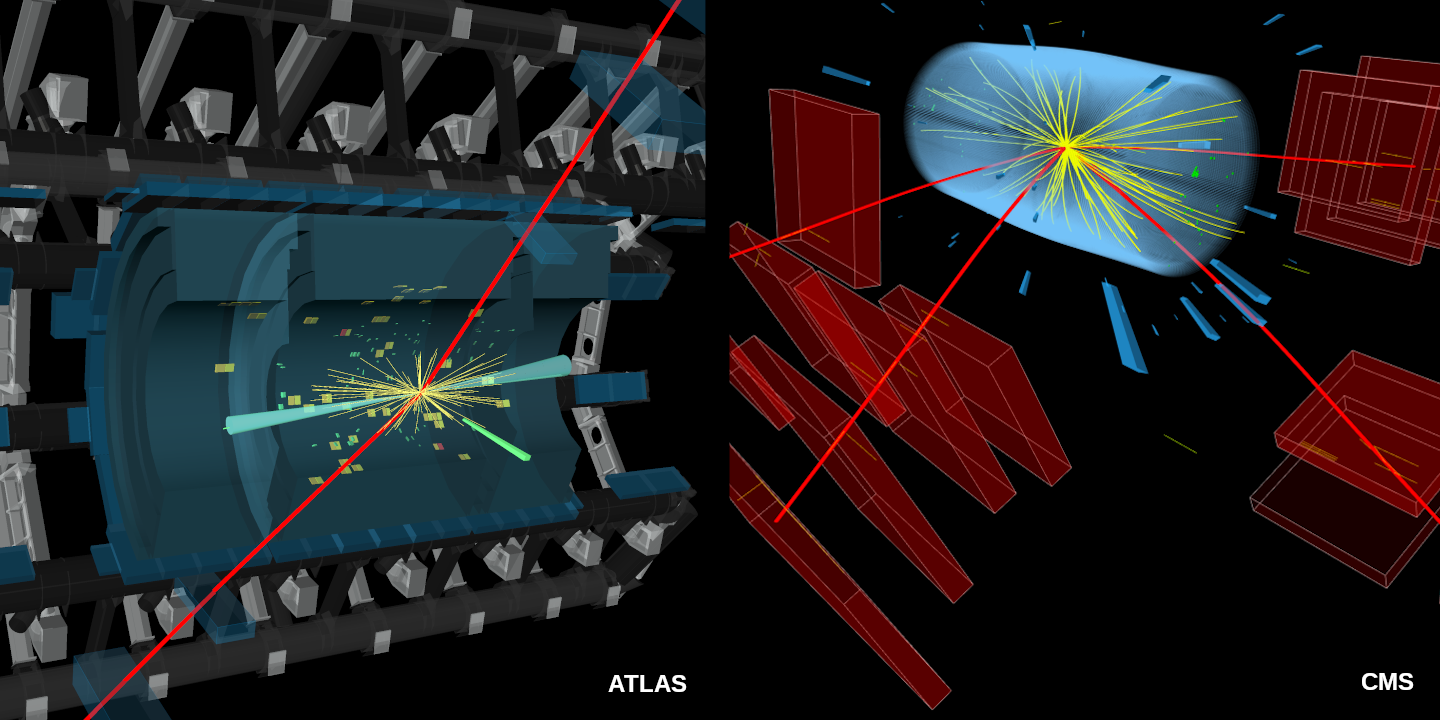
\includegraphics[width=\textwidth]{gpx/altas_cms_higs.png}
  \end{center}

\end{frame}



\begin{frame}[default]
\frametitle{noframetitle}

  \begin{itemize}
    \item Só vemos as partículas finais, pero podemos calcular a súa masa
    invariante, que é a masa da súa hipotética partícula nai. Por
    exemplo a do $Z^0 \rightarrow e^+ e^-$ ou $Z^0 \rightarrow \mu^+ \mu^-$.
  
    \item Calcúlase coa conservación da enerxía e o momento relativista:
    $$ m(Z^0) = \sqrt{ (E(\mu^+)+E(\mu^-))^2 - (\vec{p}(\mu^+)+\vec{p}(\mu^-))^2 } $$
  
    \item Calculamos a masa invariante para moitos eventos e representamos as medidas nun
    histograma. Se as partículas veñen da mesma partícula nai, veremos un
    pico no valor da súa masa.
  \end{itemize}

\end{frame}



\begin{frame}[default]
\frametitle{noframetitle}

  Datos tomados no Run 1 por ATLAS na canle $H \rightarrow \gamma \gamma$
  
  \begin{center}
  \animategraphics[width=0.6\textwidth,autoplay]{12}{gpx/higgs-gamma-gamma-cut/out-}{0}{224}
  \end{center}

\end{frame}



\subsection*{É o voso turno}
\begin{frame}
\frametitle{noframetitle}

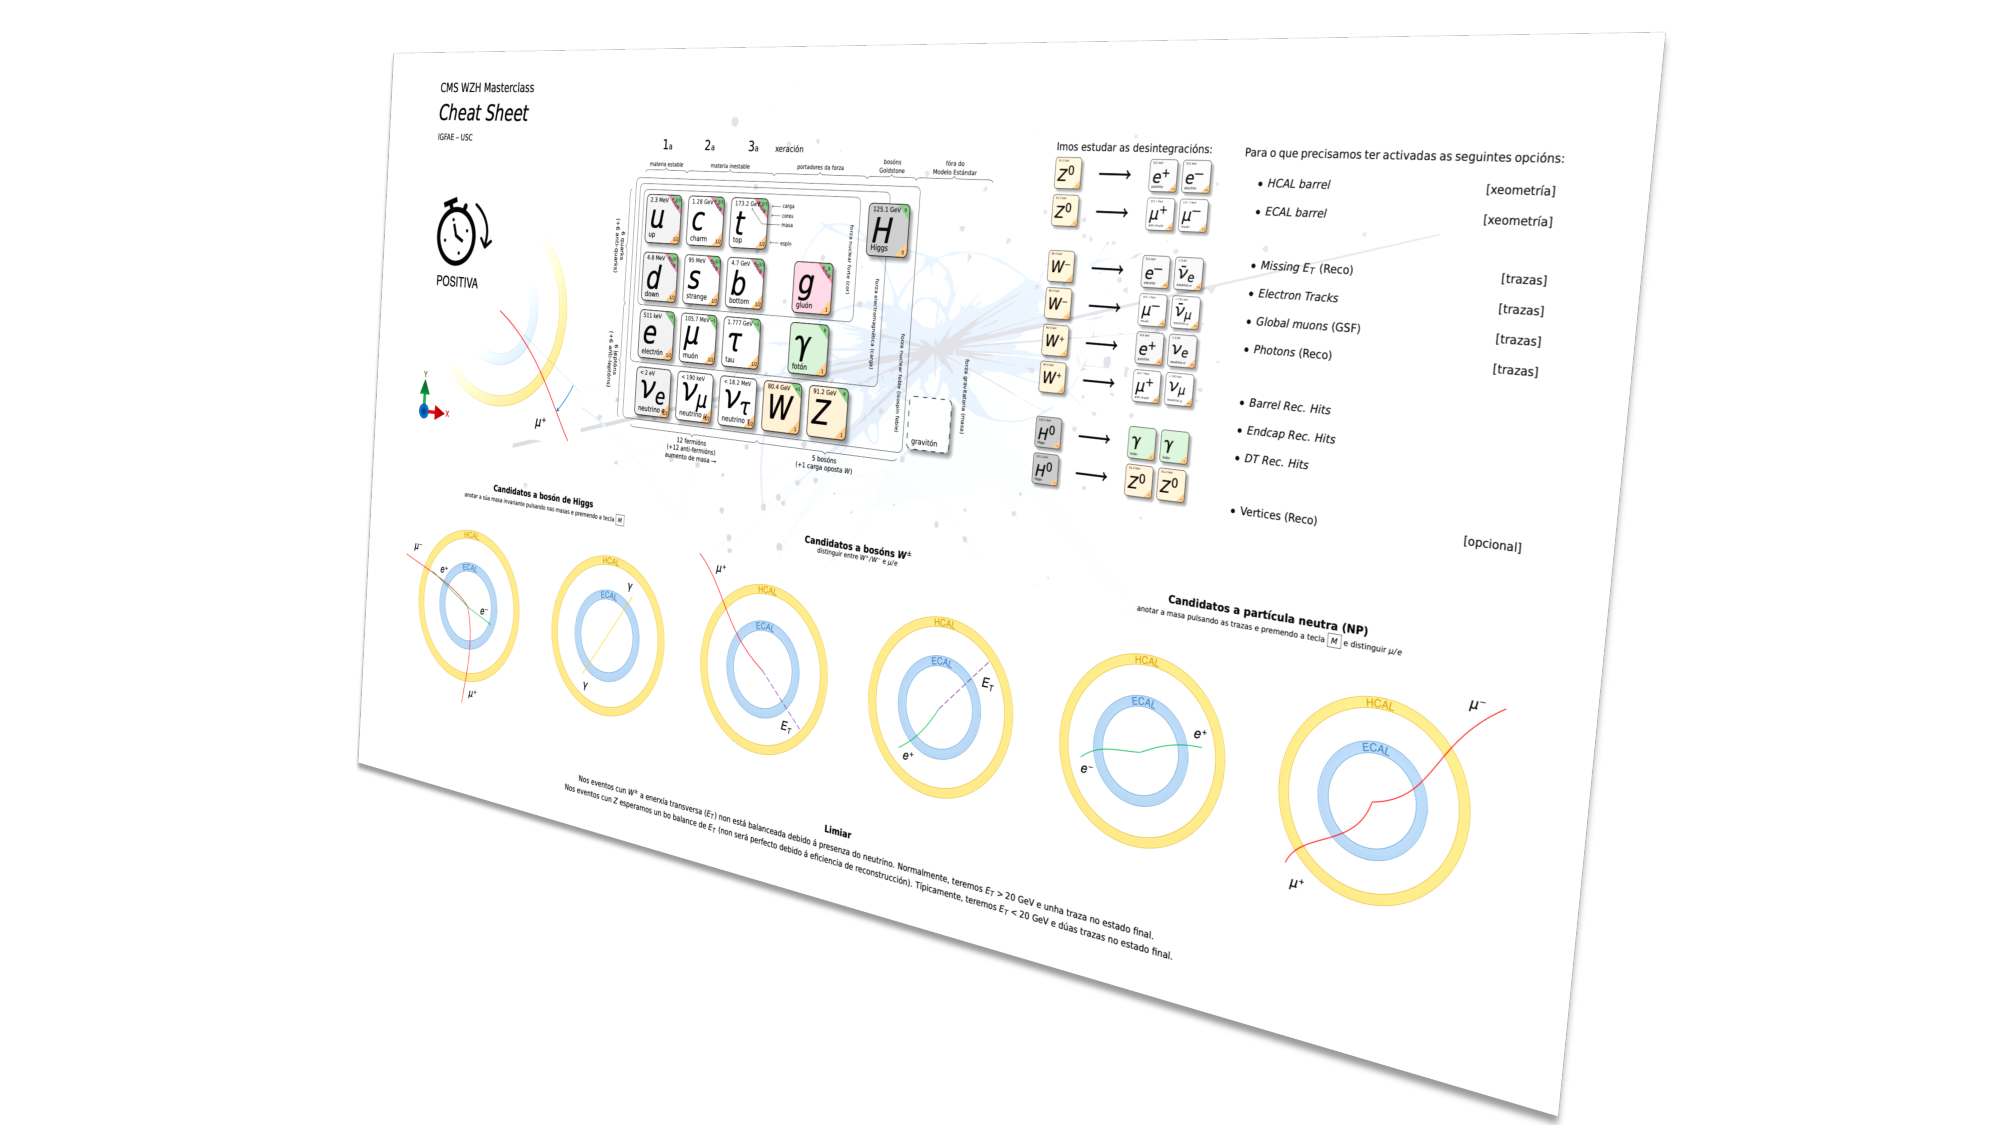
\includegraphics[scale=0.4]{gpx/cheat_sheet.pdf}

\end{frame}



\begin{frame}[plain,backgroundpicture=gpx/cms_higgs_43,overlaytoc=0.9]
  \addtocounter{framenumber}{-1}
  \hspace*{7.3cm}\begin{minipage}{8cm}
    \vspace*{1cm}
    {\Huge \fontspec{SignPainter} \textit{Grazas!}}
    
  \end{minipage}
\end{frame}



\section*{}
\subsection*{}
\begin{frame}[default,plain,backgroundpicture=gpx/revistar.pdf]
\frametitle{noframetitle}
\end{frame}



\end{document}
